実験のセットアップ
$\mu$を検出しアナログ信号に変えるために用いた装置は以下のものからなっている。
・プラスチックシンチレータ($100\times 48\times 1cm$)2枚
・プラスチックシンチレータ($120\times 5\times 1cm$)7枚
・光電子増倍管(PMT)2本
・コイル(詳細は後述)1つ
・銅板($50\times 48\times 1cm$)1つ
・MPPC及びそのための基盤(詳細は後述)7つ
・光ファイバー7本
以上の装置を次の図のように$\mu$の寿命測定(以下実験a)、$\mu$のg因子測定(以下実験b)それぞれ配置した。
実験a
\begin{figure}[h]
  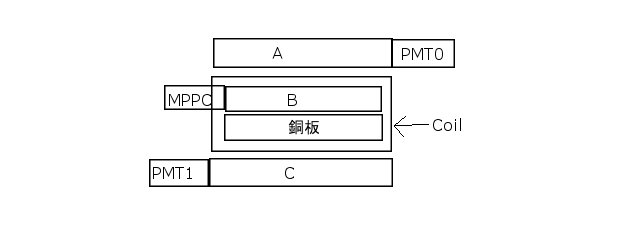
\includegraphics[width=10cm]{zikken_a.xcf}
  \caption{$\mu$の寿命測定}
\end{figure}
実験b
\begin{figure}[h]
  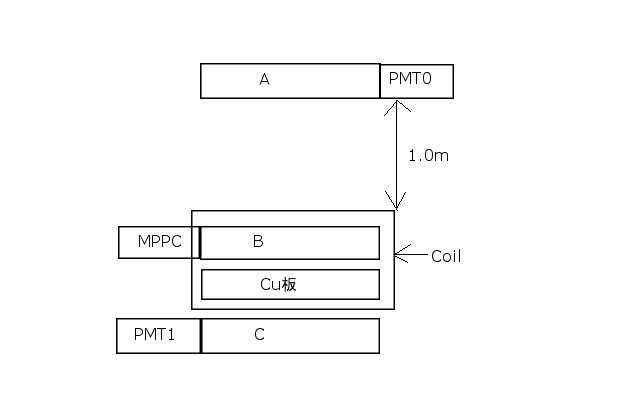
\includegraphics[width=10cm]{zikken_b.xcf}
 \caption{$\mu$のg因子測定装置}
\end{figure}
ここで、A,B,Cはいずれもプラスチックシンチレータである。
上記の装置で$\mu$は、以下のような振る舞いを行う。
1.$\mu$がどこからか降って来て、AとBを突き抜け、銅板にたどり着く。
2.銅板にたどり着いた$\mu$はエネルギーが高い場合突き抜け、Cまでたどり着くが、
あるエネルギー程度の$\mu$はCu板で止まる。
3.2で銅板で止まった$\mu$は時間が経過すると弱い相互作用によって崩壊する。
4.3で生じた陽電子がB、またはCにたどり着く。

なお、実験aとbのそれぞれのセットアップでMPPCとPMT0の距離を変えたのは、aでは$\mu$のカウント数をなるべく増やして統計誤差を減らすために狭く設定したが、bではシンチレータに対してスピンの方向が垂直な向きであることを仮定しているので、あまり上のシンチレータと銅板との間隔が狭いと斜めからの$\mu$が入り込んでしまうことも考慮して、aより広く間隔を設定した。
実験の回路図
\begin{figure}[htbm]
  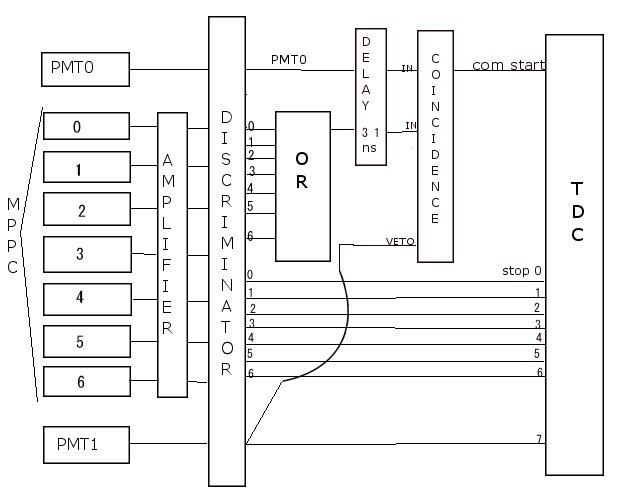
\includegraphics[width=10cm]{kairo.xcf}
  \caption{実験回路図}
\end{figure}
また、この回路図でdelay31nsを組んでいるのは、MPPCとPMT0、PMT1の信号をCOINCIDENCEでタイミングを合わせるためである。
この回路を論理記号を用いて表すと、
\begin{itemize}
$Start$信号 $(PMT0 \land MPPC)\lnot PMT1 $
$Stop$信号0~6 $ MPPC 0~6 $
$Stop$信号7 $ MPPC1 $
となる。
